\documentclass{beamer}

\mode<presentation> {
\usetheme{Madrid}
\setbeamertemplate{navigation symbols}{}
}

\usepackage{graphicx}
\usepackage{booktabs}
\usepackage[utf8]{inputenc}
\usepackage{subfigure}
\usepackage{array}
\usepackage[]{algorithm2e}
\usepackage{caption}
\usepackage{subcaption}
\usepackage{animate}

\usepackage{amsmath, amssymb}
\usepackage{bbm}
%\usepackage{algorithm}
%\usepackage{algorithmicx}
%\usepackage[noend]{algpseudocode}
%
\newcommand{\nextstate}{s^\prime}
\newcommand{\nextaction}{a^\prime}
\newcommand{\actionspace}{\mathcal{A}}
\newcommand{\statespace}{\mathcal{S}}
\newcommand{\rewardspace}{\mathcal{R}}
\newcommand{\expectation}{\mathbb{E}}
\DeclareMathOperator*{\argmax}{argmax}

\setbeamertemplate{caption}[numbered]

\newcommand{\norm}[1]{\left\lVert#1\right\rVert}

\title[Reinforcement Learning]{Reinforcement Learning}
\author[Rasmus Holm]{Rasmus Holm}
\institute[LiU]{
Linköping University \\
}
\date{\today}

\begin{document}
    %----------------------------------------------------------------------------------------
    %	INTRODUCTION SLIDES
    %----------------------------------------------------------------------------------------

    \begin{frame}
        \titlepage
    \end{frame}

    \begin{frame}
        \frametitle{Overview}
        \tableofcontents
    \end{frame}
    %----------------------------------------------------------------------------------------
    %	PRESENTATION SLIDES
    %----------------------------------------------------------------------------------------

    \section{Introduction}

    \begin{frame}
        \frametitle{Introduction}
    \end{frame}

    \begin{frame}
        \frametitle{Use Cases}

        \begin{itemize}
            \item Games
            \item Robotics
            \item Other
        \end{itemize}
    \end{frame}

    \section{Motivation}

    \begin{frame}
        \frametitle{Motivation}
    \end{frame}

    \section{The problem}

    \begin{frame}
        \frametitle{Snake}
        \centering
        \animategraphics[loop,controls,width=0.6\linewidth]{8}{./gifs/self_playing/self_playing-}{0}{41}
    \end{frame}

    \begin{frame}
        \frametitle{Snake}
        \centering
        \animategraphics[loop,controls,width=0.6\linewidth]{8}{./gifs/suicide/suicide-}{0}{19}
    \end{frame}

    \begin{frame}
        \frametitle{Snake}
        \centering
        \animategraphics[loop,controls,width=0.6\linewidth]{4}{./gifs/shortest_path/shortest_path-}{0}{55}
    \end{frame}

    \section{Theory}

    \begin{frame}
        \frametitle{The interaction loop}
        \begin{figure}[H]
            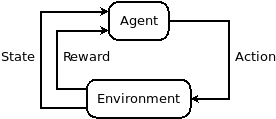
\includegraphics[width=0.8\textwidth]{../report/images/agent_env}
            \caption{The agent-environment interaction loop.}
            \label{fig:agent_env}
        \end{figure}
    \end{frame}

    \begin{frame}
        \frametitle{Markov Decision Process}

        \small
        \begin{align*}
            \actionspace & \text{: Action space} \\
            \statespace & \text{: State space} \\
            G_t &= R_{t + 1} + \gamma R_{t + 2} + \ldots = \sum_{k = 0}^{\infty} \gamma^k R_{t + k + 1} \\
            \pi(a | s) &= Pr(A_t = a | S_t = s) \\
            v_{\pi}(s) &= \expectation_\pi \left[ G_t \bigg\rvert S_t = s \right]
            = \sum_a \pi(a | s) \sum_{\nextstate, r} p(\nextstate, r | s, a) \left[ r + \gamma v_\pi(\nextstate) \right] \\
            q_{\pi}(s, a) &= \sum_{\nextstate, r} p(\nextstate, r | s, a) \left[ r + \gamma \sum_{\nextaction} \pi(\nextaction | \nextstate) q_\pi(\nextstate, \nextaction) \right] \\
            v_{\ast}(s) &= \max_a \sum_{\nextstate, r} p(\nextstate, r | s, a) \left[ r + \gamma v_\ast(\nextstate) \right] \\
            q_{\ast}(s, a) &= \sum_{\nextstate, r} p(\nextstate, r | s, a) \left[ r + \gamma \max_{\nextaction} q_\ast(\nextstate, \nextaction) \right]
        \end{align*}
        \normalsize
    \end{frame}

    \begin{frame}
        \frametitle{Policy}

        \begin{algorithm}[H]
            \KwData{State $s$, Action-value function $q$,
            Exploration rate $\epsilon \in [0, 1]$}
            Sample $u \sim U(0, 1)$

            \eIf{$u < \epsilon$}
            {
            Sample $i \sim U(\{ 1, 2, \ldots, |\actionspace| \})$

            $action = \actionspace_i$
            }
            {
            $action = \displaystyle\argmax_a q(s, a)$
            }

            \Return{$action$}
            \caption{$\epsilon$-Greedy Policy}
            \label{alg:epsilon_greedy_policy}
        \end{algorithm}
    \end{frame}

    \begin{frame}
        \frametitle{Temporal Difference Learning}

        \begin{algorithm}[H]
            \KwData{Learning rate $\alpha \in [0, 1]$, Discount factor $\gamma \in [0, 1]$}

            Initialize $\forall_{a \in \actionspace, s \in \statespace} Q(a, s)$ arbitrarily and $Q$(terminal state, $\cdot$) = 0

            \For{each episode}{

            Initialize $S$

            Choose $A$ from $S$ using policy $\pi$ ($\epsilon$-greedy) derived from $Q$

            \While{$S$ is non-terminal state}{

            Perform action $A$, observe state $S^\prime$ and reward $R$

            Choose $A^\prime$ from $S^\prime$ using policy $\pi$ ($\epsilon$-greedy) derived from $Q$

            Update $Q(S, A)$ based on $(S, A, R, S^\prime, A^\prime, \pi, \alpha, \gamma$)

            $S = S^\prime$

            $A = A^\prime$
            }
            }

            \Return{$Q$}
            \caption{TD Learning Algorithm}
            \label{alg:td_learning}
        \end{algorithm}
    \end{frame}

    \begin{frame}
        \begin{figure}[ht]
            \centering
            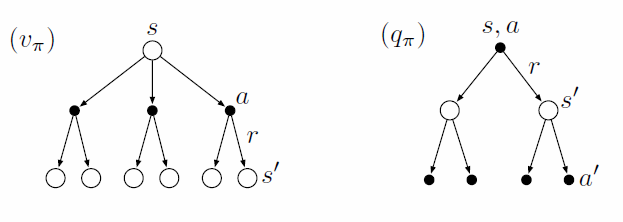
\includegraphics[width=\linewidth]{./images/backup_diagrams.PNG}
            \caption{Backup diagrams for state-value function and action-value function.}
            \label{fig:backup_diagrams}
        \end{figure}
    \end{frame}

    \section{Results}

    \begin{frame}
        \frametitle{Q-Learning}
        \begin{figure}
            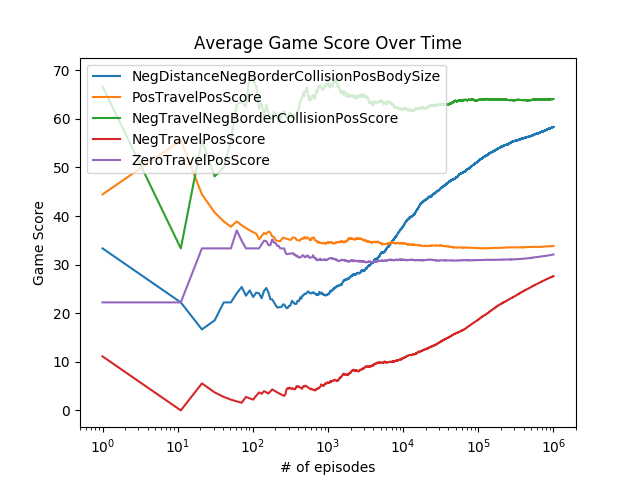
\includegraphics[width=0.5\textwidth]{../images/qlearning/reward/42/reward_qlearning_board_state_average_game_score_over_time.png}
            \hfill
            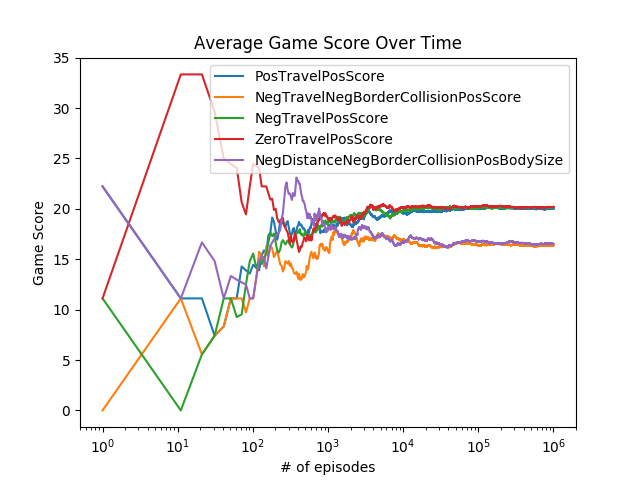
\includegraphics[width=0.5\textwidth]{../images/qlearning/reward/42/reward_qlearning_directional_state_average_game_score_over_time.png}
            \caption{Results generated by Q-Learning. Upper: Board state. Lower: Directional State.}
            \label{fig:reward_result_qlearning}
        \end{figure}
    \end{frame}

    \begin{frame}
        \frametitle{Sarsa}
        \begin{figure}
            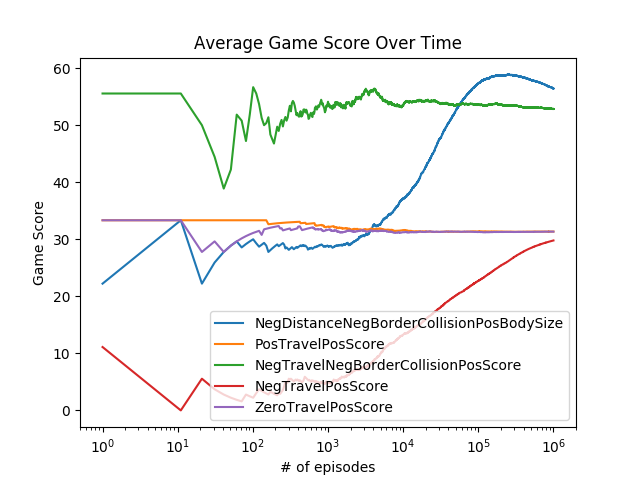
\includegraphics[width=0.5\textwidth]{../images/sarsa/reward/42/reward_sarsa_board_state_average_game_score_over_time.png}
            \hfill
            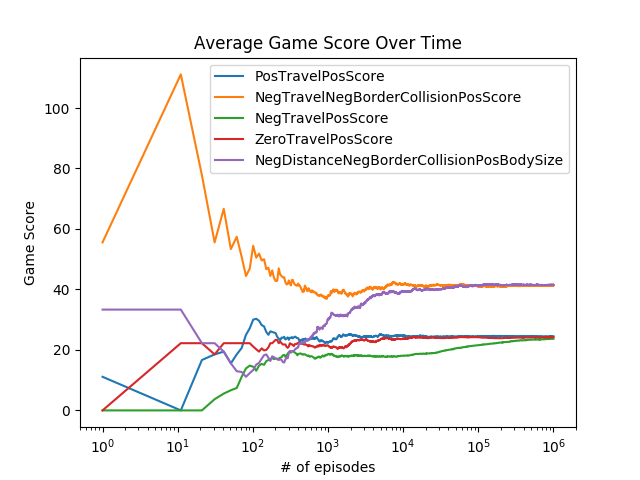
\includegraphics[width=0.5\textwidth]{../images/sarsa/reward/42/reward_sarsa_directional_state_average_game_score_over_time.png}
            \caption{Results generated by Sarsa. Left: Board state. Right: Directional State.}
            \label{fig:reward_result_sarsa}
        \end{figure}
    \end{frame}

    \begin{frame}
        \frametitle{Q-Learning}
        \begin{figure}
            \centering
            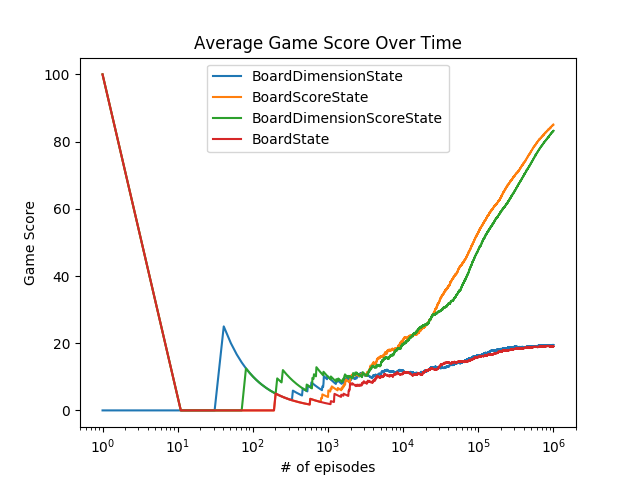
\includegraphics[width=0.8\textwidth]{../images/qlearning/info_augmentation/123/board_state_average_game_score_over_time.png}
            \caption{Board state with different augmented information.}
            \label{fig:info_augmentation_board_state}
        \end{figure}
    \end{frame}

    \begin{frame}
        \frametitle{Q-Learning}
        \begin{figure}[ht]
            \centering
            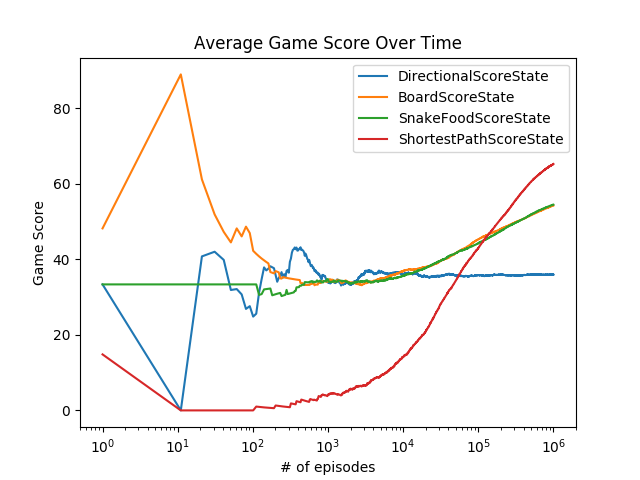
\includegraphics[width=0.8\linewidth]{../images/qlearning/state/42/state_qlearning_average_game_score_over_time.png}
            \caption{Performance of state representations trained using Q-learning.}
            \label{fig:state_qlearning}
        \end{figure}
    \end{frame}

    \begin{frame}
        \frametitle{Q-Learning}
        \begin{table}[ht]
            \centering
            \begin{tabular}{ | l | l | l | }
                \hline
                State & Avg. Score & Std. Deviation \\ \hline
                ShortestPathScoreState & 129.50 & 51.11 \\ \hline
                BoardScoreState & 103.12 & 17.73 \\ \hline
                DirectionalScoreState & 66.12 & 64.328 \\ \hline
                SnakeFoodScoreState & 104.12 & 20.08 \\ \hline
                Random Agent & 20.13 & 46.47 \\
                \hline
            \end{tabular}
            \caption{Test performance over 10000 episodes.}
            \label{table:state_qlearning}
        \end{table}
    \end{frame}

    \begin{frame}
        \frametitle{Sarsa}
        \begin{figure}[ht]
            \centering
            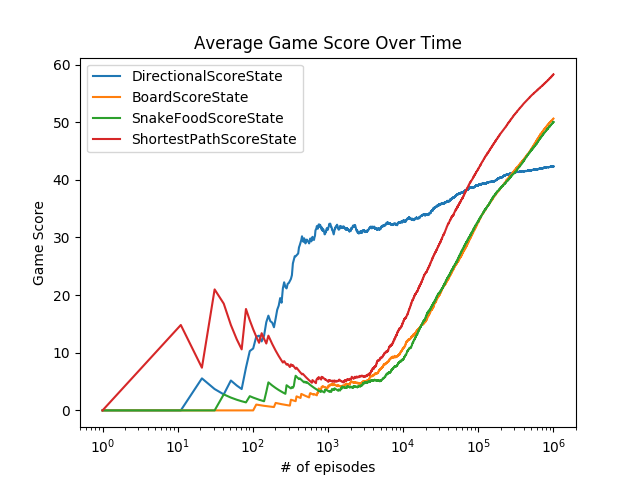
\includegraphics[width=0.8\linewidth]{../images/sarsa/state/42/state_sarsa_average_game_score_over_time.png}
            \caption{Performance of state representations trained using Sarsa.}
            \label{fig:state_sarsa}
        \end{figure}

    \end{frame}

    \begin{frame}
        \frametitle{Sarsa}
        \begin{table}[ht]
            \centering
            \begin{tabular}{ | l | l | l | }
                \hline
                State & Avg. Score & Std. Deviation \\ \hline
                ShortestPathScoreState & 118.59 & 38.95 \\ \hline
                BoardScoreState & 101.02 & 10.05 \\ \hline
                DirectionalScoreState & 72.16 & 71.60 \\ \hline
                SnakeFoodScoreState & 101.02 & 10.05 \\ \hline
                Random Agent & 20.13 & 46.47 \\
                \hline
            \end{tabular}
            \caption{Test performance over 10000 episodes.}
            \label{table:state_sarsa}
        \end{table}
    \end{frame}

    \section{Conclusion}

    \begin{frame}
        \frametitle{Conclusion}

    \end{frame}

    \begin{frame}
        \Huge{\centerline{The End}}
    \end{frame}

\end{document}
